%%%%%%%%%%%%%%%%%%%%%%%%%%%%%%%%%%%%%%%%%
% Short Sectioned Assignment LaTeX Template Version 1.0 (5/5/12)
% This template has been downloaded from: http://www.LaTeXTemplates.com
% Original author:  Frits Wenneker (http://www.howtotex.com)
% License: CC BY-NC-SA 3.0 (http://creativecommons.org/licenses/by-nc-sa/3.0/)
%%%%%%%%%%%%%%%%%%%%%%%%%%%%%%%%%%%%%%%%%

% \documentclass[paper=a4, fontsize=11pt]{scrartcl} % A4 paper and 11pt font size
\documentclass[11pt, a4paper]{book}
\usepackage[T1]{fontenc} % Use 8-bit encoding that has 256 glyphs
\usepackage[utf8]{inputenc}
\usepackage{fourier} % Use the Adobe Utopia font for the document - comment this line to return to the LaTeX default
\usepackage{listings} % para insertar código con formato similar al editor
\usepackage[spanish, es-tabla]{babel} % Selecciona el español para palabras introducidas automáticamente, p.ej. "septiembre" en la fecha y especifica que se use la palabra Tabla en vez de Cuadro
\usepackage{url} % ,href} %para incluir URLs e hipervínculos dentro del texto (aunque hay que instalar href)
\usepackage{graphics,graphicx, float} %para incluir imágenes y colocarlas
\usepackage[gen]{eurosym} %para incluir el símbolo del euro
\usepackage{cite} %para incluir citas del archivo <nombre>.bib
\usepackage{enumerate}
\usepackage{hyperref}
\usepackage{graphicx}
\usepackage{tabularx}
\usepackage{booktabs}

\usepackage[table,xcdraw]{xcolor}
\hypersetup{
	colorlinks=true,	% false: boxed links; true: colored links
	linkcolor=black,	% color of internal links
	urlcolor=cyan		% color of external links
}
\renewcommand{\familydefault}{\sfdefault}
\usepackage{fancyhdr} % Custom headers and footers
\pagestyle{fancyplain} % Makes all pages in the document conform to the custom headers and footers
\fancyhead[L]{} % Empty left header
\fancyhead[C]{} % Empty center header
\fancyhead[R]{Marcos Romero Martín} % My name
\fancyfoot[L]{} % Empty left footer
\fancyfoot[C]{} % Empty center footer
\fancyfoot[R]{\thepage} % Page numbering for right footer
%\renewcommand{\headrulewidth}{0pt} % Remove header underlines
\renewcommand{\footrulewidth}{0pt} % Remove footer underlines
\setlength{\headheight}{13.6pt} % Customize the height of the header

\usepackage{titlesec, blindtext, color}
\definecolor{gray75}{gray}{0.75}
\newcommand{\hsp}{\hspace{20pt}}
\titleformat{\chapter}[hang]{\Huge\bfseries}{\thechapter\hsp\textcolor{gray75}{|}\hsp}{0pt}{\Huge\bfseries}
\setcounter{secnumdepth}{4}
\usepackage[Lenny]{fncychap}

\usepackage{amssymb}
\usepackage{pifont}
\usepackage{adjustbox}
\usepackage{float}

\usepackage{algorithm}
\usepackage[noend]{algpseudocode}
\usepackage{amsmath}  % Paquete necesario para usar \text{} dentro de ecuaciones
\usepackage{amsfonts}
\usepackage{subcaption}  % Para las imágenes en formato 2x2
\usepackage{pgfgantt}

\begin{document}

	% Plantilla portada UGR
	\begin{titlepage}
\newlength{\centeroffset}
\setlength{\centeroffset}{-0.5\oddsidemargin}
\addtolength{\centeroffset}{0.5\evensidemargin}
\thispagestyle{empty}

\noindent\hspace*{\centeroffset}\begin{minipage}{\textwidth}

\centering
\includegraphics[width=0.9\textwidth]{logos/logo_ugr.jpg}\\[1.4cm]

\textsc{ \Large TRABAJO FIN DE GRADO\\[0.2cm]}
\textsc{ GRADO EN INGENIERIA INFORMATICA}\\[1cm]

{\Huge\bfseries Mejoras en un sistema de defensa móvil ante ataques de Internet \\}
\noindent\rule[-1ex]{\textwidth}{3pt}\\[3.5ex]
{\large\bfseries Rotación de servidores como defensa dinámica }
\end{minipage}

\vspace{2.5cm}
\noindent\hspace*{\centeroffset}
\begin{minipage}{\textwidth}
\centering

\textbf{Autor}\\ {Marcos Romero Martín}\\[2.5ex]
\textbf{Director}\\ {Juan Julián Merelo Guervós}\\[2cm]
\includegraphics[width=0.3\textwidth]{logos/etsiit_logo.png}\\[0.1cm]
\textsc{Escuela Técnica Superior de Ingenierías Informática y de Telecomunicación}\\
\textsc{---}\\
Granada, noviembre de 2023
\end{minipage}
\end{titlepage}


	% Plantilla prefacio UGR
	\thispagestyle{empty}

\begin{center}
{\large\bfseries Mejoras en un sistema de defensa móvil ante ataques de Internet \\ Rotación de servidores como defensa dinámica }\\
\end{center}
\begin{center}
	Marcos Romero Martín\\
\end{center}

%\vspace{0.7cm}

\vspace{0.5cm}
\noindent\textbf{Palabras clave}: \textit{software libre}, \textit{moving target defense},  \textit{rotacion}
\vspace{0.7cm}

\noindent\textbf{Resumen}\\
	
La creciente sofisticación de los ataques a servicios web ha puesto en evidencia las limitaciones de las defensas tradicionales basadas en sistemas estáticos, donde los atacantes tienen tiempo suficiente para estudiar y explotar vulnerabilidades.

En este contexto, la necesidad de un Moving Target Defense (MTD) surge como una solución efectiva para aumentar la defensa. Al cambiar dinámicamente el entorno operativo, el MTD introduce imprevisibilidad, dificultando que los atacantes obtengan información precisa sobre la infraestructura a comprometer.

El documento presenta la implementación y evaluación de un sistema de defensa dinámica (MTD) para servidores web, con el objetivo de mejorar la seguridad ante ataques. A través de una revisión del estado del arte, se establece el contexto teórico que sustenta la solución propuesta. La planificación del proyecto se estructura mediante historias de usuario, siguiendo un desarrollo ágil. Posteriormente, se describe la implementación técnica del MASS, un sistema que rota servidores Apache y Nginx utilizando contenedores Docker, seguido de pruebas que evalúan el rendimiento, el consumo de recursos y la resistencia a vulnerabilidades. Aportando una solución autocontenida de código abierto a dicho problema. Finalmente, se presentan conclusiones y sugerencias para futuras mejoras, como la integración de un sistema de detección de intrusos (IDS) y la restauración desde snapshots.


\cleardoublepage

\begin{center}
	{\large\bfseries Same, but in English}\\
\end{center}
\begin{center}
	Marcos Romero Martín\\
\end{center}
\vspace{0.5cm}
\noindent\textbf{Keywords}: \textit{open source}, \textit{floss}, \textit{moving target defense},  \textit{rotation}
\vspace{0.7cm}

\noindent\textbf{Abstract}\\
The growing sophistication of attacks on web services has highlighted the limitations of traditional defenses based on static systems, where attackers have enough time to study and exploit vulnerabilities.

In this context, the need for a Moving Target Defense (MTD) emerges as an effective solution to increase defense. By dynamically changing the operating environment, MTD introduces unpredictability, making it difficult for attackers to obtain accurate information about the infrastructure to be compromised.

The paper presents the implementation and evaluation of a dynamic defense system (MTD) for web servers, with the objective of improving security against attacks. Through a review of the state of the art, the theoretical context that supports the proposed solution is established. The project planning is structured by means of user stories, following an agile development. Subsequently, the technical implementation of MASS, a system that rotates Apache and Nginx servers using Docker containers, is described, followed by tests that evaluate performance, resource consumption and vulnerability resistance. Providing a self-contained open source solution to that problem. Finally, conclusions and suggestions for future improvements are presented, such as the integration of an intrusion detection system (IDS) and restoration from snapshots.

\cleardoublepage

\thispagestyle{empty}

\noindent\rule[-1ex]{\textwidth}{2pt}\\[4.5ex]

D. \textbf{Juan Julián Merelo Guervós}, Profesor del departamento de Ingeniería de Computadores, Automática y Robótica de la Universidad de Granada.

\vspace{0.5cm}

\textbf{Informo:}

\vspace{0.5cm}

Que el presente trabajo, titulado \textit{\textbf{Mejoras en un sistema de defensa móvil ante ataques de Internet}},
ha sido realizado bajo mi supervisión por \textbf{Marcos Romero Martín}, y autorizo la defensa de dicho trabajo ante el tribunal
que corresponda.

\vspace{0.5cm}

Y para que conste, expiden y firman el presente informe en Granada a septiembre de 2024.

\vspace{1cm}

\textbf{El director: }

\vspace{5cm}

\noindent \textbf{Juan Julián Merelo Guervós}

\chapter*{Agradecimientos}
A mi familia y amigos, por aguantarme, que no es poco. También quiero agradecer, en especial, a JJ por tutorizar este trabajo.

	% Índice de contenidos
	\newpage
	\tableofcontents

	% Índice de imágenes y tablas
	\newpage
	\listoffigures

	% Si hay suficientes se incluirá dicho índice
	\listoftables 
	\newpage

	% Introducción 
	\chapter{Introducción}

Los servidores son la cara visible de internet, por ejemplo, actualmente hay alrededor de 12.1 millones de servidores web activos en el mundo \cite{netcraft-agosto23}. Estos servidores son el objetivo de muchos ataques, ya que son la puerta de entrada a los datos de los usuarios.\cite{breaches-2023} Por ello, es importante que los servidores estén protegidos ante ataques, y que en caso de que se produzca un ataque, el servidor sea capaz de recuperarse y seguir ofreciendo servicio.

Hay diferentes tecnologías para aumentar la seguridad, por ejemplo los \textit{firewalls}, listas de control de acceso (ACL), \textit{firewalls} para web (WAF), \textit{Honeypots}, etc. Sin embargo, estas técnicas tienen algo en común, y es que son estáticas (se definen mediante configuraciones predefinidas). Existen otras tecnologías que pueden tomar acciones basadas en eventos como los sistemas de prevención de intrusión (IPS) o los antivirus en tiempo real. Sin embargo, ninguna de las técnicas anteriores cambia el entorno para defenderse del atacante, es decir, en el caso de sufrir una intrusión y ser mitigada, el servidor sigue estando en el mismo estado que antes del ataque. Esto es un problema, ya que la vulnerabilidad sigue estando presente, y hasta que no sea arreglada por el administrador, el atacante puede volver a intentar explotarla.
 
Para solucionar lo anterior, se introduce un concepto llamado \textit{moving target defense}\cite{big-state-of-art} (MTD de ahora en adelante), el cual se refiere a una estrategia de seguridad dinámica que implica cambiar la configuración o distribución de un sistema para dificultar los ataques y proteger contra las amenazas. Esta estrategia busca hacer que los sistemas sean menos predecibles para los atacantes al cambiar las condiciones bajo las cuales operan. No busca reemplazar a las técnicas existentes, sino complementarlas.

Con este trabajo se pretende facilitar el trabajo a los investigadores, implementando uno de los últimos MTD como herramienta de código abierto que les permita probar y evaluar este tipo de técnicas. Además se pretende realizar diferentes comparativas para evaluar dicha implementación, realizando así una aportación a dicha línea de investigación. Para llevar a cabo todo lo anterior, nos apoyaremos en el desarrollo ágil.

Este proyecto es software libre, y está liberado con la licencia\cite{gplv3} en \url{https://github.com/marcosrmartin/MTD_Server}.

	% Descripción del problema y hasta donde se llega
	% \input{secciones/02_descripcion}

	% Estado del arte
	% 	1. Crítica al estado del arte
	% 	2. Propuesta
	\chapter{Estado del arte}

El concepto MTD se empieza a popularizar de forma teórica en informática (ya que no es exclusiva de esta) hace unos 10 años. Se han realizado investigaciones aplicándolo a diferentes ámbitos de la informática, donde con el paso de las investigaciones se ha ido creando una clasificación de las diferentes técnicas de MTD \cite{big-state-of-art}.
\begin{figure}[h]
    \centering
    \includegraphics[width=\linewidth]{./imagenes/busquedasMTD.png}
    \caption{Investigaciones sobre MTD a lo largo del tiempo}
\end{figure}

A continuación vamos a hacer una revisión sobre los aspectos más importantes de los MTD, como son la clasificación y limitaciones. Además haremos un repaso sobre las implementaciones que se han realizado sobre servidores web, ya que es el objetivo de este trabajo.

\section{Clasificación}
Cuando queremos implementar un MTD, necesitamos elegir el componente más viable o donde necesitamos más protección.

\textbf{Qué mover}: debería ser un componente o atributo que habilite un vector de ataque. Por ejemplo, pueden ser una IP \cite{MTD-SDN+decoy}\cite{MTD-ipshuffling+honeypots}\cite{MTD-POC-empresa}, servidor web \cite{MTD-DARE}\cite{MTD-MORE+DARE+Java}, sistema operativo \cite{MTD-MORE+DARE+Java}, direcciones de memoria \cite{MTD-ASR}, base de datos \cite{MTD-arab}, WAF \cite{MTD-WAF}, VM \cite{MTD-POC-empresa}\cite{MTD-DARE}\cite{SCIT-base}, etc.

\textbf{Cómo moverlo}: una vez se ha seleccionado el componente, hay que determinar como cambiarlo, para esto hay tres opciones diferentes:
\begin{itemize}
    \item Mezcla: se cambia un componente por otro, los ejemplos de componentes incluyen direcciones IP de un servidor o las variables de entorno de un sistema.
    \item Diversidad: tiene componentes diferentes que realizan la misma tarea, por ejemplo, en vez de varios servidores Apache como servidores web, tiene un Apache y dos Nginx.
    \item Redundancia: tener componentes repetidos para asegurar que, si uno falla o es comprometido, otros pueden tomar su lugar o mitigar el impacto del ataque. 
\end{itemize}

\begin{figure}[h]
    \centering
    \includegraphics[width=\linewidth]{./imagenes/tiposmovimientos.png}
    \caption{Formas de mover un componente}
\end{figure}

\textbf{Cuándo moverlo}: una vez que se ha seleccionado el componente y la forma de moverlo, hay que determinar cuando moverlo. Hay dos opciones:
\begin{itemize}
    \item Por tiempo (proactivo): se mueve el componente de forma periódica, independientemente de si se ha detectado un ataque o no. El periodo no tiene por qué ser fijo, puede ser aleatorio o entre un rango de tiempo.
    \item Por evento (reactivo): se mueve el componente cuando se detecta un ataque o un fallo en el sistema, la forma de detectarlo puede ser machine learning\cite{MTD-ML}, uso de IPS\cite{Design-Generic-Intrusion-Tolerant-Architecture}, un WAF \cite{MTD-WAF}, etc.
\end{itemize}

Esta clasificación no es excluyente, es decir se pueden combinar diferentes opciones. Por ejemplo, se pueden combinar las dos opciones de cuando moverlo (creando una opción híbrida) con todas las opciones de como moverlo. La mayoría de veces una implementación combina varios de estas \cite{MTD-MORE+DARE+Java}\cite{MTD-DARE}\cite{MTD-arab}, aunque que exista esta posibilidad no quiere decir que se deban de mezclar todas las opciones posibles, ya que podrían dar configuraciones menos seguras o eficientes que al utilizar menos opciones \cite{MTD-comparativa-gorda}.

\section{Servidores web}
Los MTD basados en servidores web no son una de las principales líneas de investigación, ya que son más difíciles de adaptar a un entorno de producción, no hay consenso sobre ellos y no han demostrado tener resultados tan eficaces como otras líneas (SDN o \textit{IP shuffling}). Aun así, se han realizado varias implementaciones sobre estos, nos centraremos en aquellos que rotan los servidores que se utilizan, comenzando por el DARE (\textit{Dynamic Application Rotation Environment for Moving Target Defense}) este se basa en la estrategia utilizada por el MORE (\textit{Multiple Operating System Rotational Environment MTD})\cite{MORE}, la cual consiste en ir cambiando la máquina que recibe el tráfico mediante IP. DARE lo implementa en los puertos, esta consiste en rotar un servidor Nginx\cite{nginx} con uno Apache\cite{apache}, los cuales están en la misma máquina, para servir una página web estática. Esto lo logran utilizando un script como servicio el cual cambia la entrada de Iptables\cite{iptables} para apuntar a un puerto u otro.

El problema de DARE es que al actualizar el firewall, se perdía mucha disponibilidad al reiniciar el servicio, por lo que a partir de esta, surge \textit{DARE IMproved} (DIM). Este utiliza la misma estrategia que DARE, pero utiliza un script en Python el cual altera Iptables, pero no reinicia el servicio. Esto es posible, ya que si una regla está definida correctamente en Iptables, no es necesario reiniciarlo para que entre en funcionamiento, llevando la disponibilidad hasta el 98\%. Otra mejora que hace DIM respecto a DARE, es que redirige el tráfico a los servidores mediante el \textit{loopback}, lo que permite que los servidores no sean accesibles desde fuera de la máquina. Con estas mejoras se consiguieron aumentar la disponibilidad, rendimiento y la seguridad.

A pesar de las mejoras llevadas a cabo, la disponibilidad sigue sin ser suficiente, algunos sitios web deben tener una disponibilidad del 99.99\% para cumplir con el acuerdo de nivel de servicio (SLA)\cite{SLA}, al modificar Iptables, los paquetes que estaban siendo procesados por el servidor son descartados automáticamente. Por lo que surge \textit{Mutable Asymmetric web Server Security} (MASS), el cual está basado en las implementaciones anteriores, con las siguientes mejoras:
\begin{itemize}
    \item Utiliza Firewalld\cite{firewalld}: es una alternativa a Iptables, la cual tampoco reinicia el servicio. Además, este puede controlar el flujo de paquetes, por lo que mientras que un servidor está siendo cambiado, los paquetes son almacenados en una cola para ser enviados al acabar el cambio.
    \item Uso de contenedores: ahora cada servidor está en un contenedor diferente, lo que aumenta el aislamiento, ya que si anteriormente si un servidor era comprometido, toda la máquina lo era también.
    \item Reencarnación de contenedores: esta técnica consiste en que una vez que un contenedor es cambiado por el otro contenedor, en vez de mantenerlo o comprobar si ha sido comprometido, es destruido directamente, para volver a crear un contenedor nuevo a partir de una imagen base.
\end{itemize}

Alejándose de la línea anterior, otra implementación es la de Philip Tibom y Max Buck\cite{MTD-gotemburgo}, en la que utilizan nodos de Kubernetes\cite{kubernetes} para implementar el MTD. Esta configuración consigue un 100\% de disponibilidad. Utiliza \textit{VM shufflig}, cambiando los nodos entre diferentes ubicaciones físicas y su IP. Está preparado para utilizar distintas imágenes de Docker en diferentes nodos.

El SCIT (\textit{Self Cleansing Intrusion Tolerance})\cite{SCIT-base} es otra tecnología vinculada a los servidores web. Esta estrategia se basa en la reencarnación de un componente, similar a lo que realiza MASS. En 2011, se publicó un estudio\cite{SCIT-cloud}, que compartía estructura con el trabajo de Philip Tibom y Max Buck; sin embargo, en este caso se implementaba el SCIT. Es notable mencionar que, pese a los 11 años transcurridos desde ambas investigaciones, no se ha liberado ningún software de código abierto que emulase dicha implementación.


\section{Limitaciones}
A pesar de las diferentes investigaciones e implementaciones que existen, muchas tienen en común algunas malas prácticas y clichés que se repiten, dando lugar a un análisis erróneo de los resultados. Estas prácticas son:
\begin{itemize}
    \item Pruebas de explotación pobres: la evaluación de la defensa se suele centrar en la fase de reconocimiento, para después utilizar un único \textit{exploit} en la explotación por componente, esto hace las pruebas más fáciles, pero no da una visión realista de la seguridad, ya que utiliza un único vector de ataque, el cual no varía el tiempo que se tarda en explotar la vulnerabilidad.
    \item MTD por eventos o híbridos dejados atrás: las investigaciones e implementaciones se suelen centrar en MTD proactivos, ya que una de las características que se le atribuye a los MTD es que son inseguros por defecto. Por lo que las líneas principales de investigación se centran en mantener el rendimiento, ofuscar el reconocimiento y reducir el tiempo que un componente es vulnerable. Si bien es cierto que los MTD proactivos pueden cumplir con estos objetivos y la mayor parte de la investigación debería seguir esa línea, dejar de lado los eventos se aleja de una solución realista, por un ejemplo tan sencillo como que en un MTD con diversidad o redundancia de servidores, uno de ellos esté caído y se le siga mandando tráfico.
    \item Aumento de la superficie de ataque: en determinados MTD proactivos la rotación de un componente puede aumentar las brechas de seguridad\cite{MTD-critica}, este es un problema intrínseco a esta tecnología, que se suele pasar por alto en la mayoría de investigaciones. Se podrían dar las siguientes situaciones como ejemplo:
    \begin{enumerate}
        \item Tenemos un componente seguro y otro inseguro: si rotamos entre ellos cada cierto tiempo, el sistema será vulnerable la mitad del tiempo. La solución realista sería dejar de cambiar al vulnerable al detectar el ataque.
        \item Si tenemos dos componentes seguros: el sistema no será vulnerable nunca, si los componentes son diferentes uno rendirá mejor que el otro. La solución realista sería mantener el componente que mejor rendimiento tenga, y si los componentes son iguales, no haría falta rotarlos, una configuración estática sería más óptima.
        \item Tenemos dos componentes inseguros: el sistema será vulnerable siempre. La solución realista sería realizar cambios constantemente hasta parchear las vulnerabilidades, que serían dos en vez de una.
    \end{enumerate}
    Como hemos dicho antes estos ejemplos no aplican a todas las tecnologías MTD, pero son uno de los problemas de raíz de esta tecnología.
    \item Atribuir la seguridad al cambio erróneamente: es decir realizamos una rotación entre diferentes componentes, pero el cambio no es gracias a utilizar un componente diferente. Un ejemplo, tenemos una vulnerabilidad que causa una denegación de servicio (DoS) en un servidor, esta tarda 30 s en empezar a funcionar y 60 s en dejar el servidor caído. Si realizamos cambios cada 15 s entre el servidor vulnerable y uno seguro (reiniciando el servidor al cambiarlo), el servidor nunca estará caído, pero no es gracias a la rotación, sino al reinicio. Si realizáramos la rotación entre dos servidores vulnerables, el servidor tampoco estaría caído, ya que el tiempo de explotación es mayor que el del cambio de componente.
    \item Falta de código \textit{opensource}: apenas hay código abierto sobre los MTD, esto hace que sea difícil replicar los resultados de las investigaciones, ya que no se puede saber si se ha implementado correctamente o no. Además de retrasar la investigación al tener que reinventar la rueda y no poder realizar comparativas entre soluciones.
\end{itemize}

\section{Analogías}

Alexander Bajic y Georg T. Becker listaron una serie de analogías\cite{MTD-critica} con los ejemplos anteriores:
\begin{itemize}
    \item El combate aéreo y bandada de pájaros: en un combate aéreo, un piloto debe hacer maniobras impredecibles para no ser un blanco fácil. Esta situación ilustra cómo las tácticas de seguridad de TI actuales son estáticas, como esperar en un búnker. Algunas empresas usan la analogía de una bandada de pájaros, donde cada ave se mueve constantemente, dificultando que un depredador ataque a una específica.
    \item La caza del ciervo: Un ciervo en movimiento puede eludir a un cazador que lo persigue. Sin embargo, si el cazador espera en un punto, dicho movimiento es lo que lo pone en peligro. Es vital considerar no solo cómo este beneficia a la defensa, sino también cómo podría beneficiar al atacante. Un ejemplo de esto es el aumento de superficie de ataque que se mencionó anteriormente.
    \item El trilero: una bola se esconde bajo uno de los tres cubiletes que se mueven rápidamente. Sin embargo, este juego suele ser un engaño, ya que el operador manipula sigilosamente la bola. Aunque el movimiento de los cubiletes puede no ser el factor de seguridad en la MTD, otros aspectos de la defensa sí lo son.
\end{itemize}

\begin{figure}[h]
    \centering
    \begin{minipage}{.3\textwidth}
        \centering
        \includegraphics[width=\linewidth]{./imagenes/bandada.jpg}
        \caption{Bandada de pájaros}
    \end{minipage}
    \hfill
    \begin{minipage}{.3\textwidth}
        \centering
        \includegraphics[width=\linewidth]{./imagenes/caza.jpg}
        \caption{Cazador esperando que el ciervo se ponga a tiro}
    \end{minipage}
    \hfill
    \begin{minipage}{.3\textwidth}
        \centering
        \includegraphics[width=\linewidth]{./imagenes/trilero.jpg}
        \caption{Trilero}
    \end{minipage}
\end{figure}

	
	\chapter{Planificación}
En este capítulo se abordarán aspectos esenciales para el desarrollo del proyecto. Se explicara el \textit{midset} y metodología utilizados para establecer y desarrollar los objetivos. Se presentan las historias de usuario que guiarán el desarrollo e hitos como objetivos concretos y como cumplirlos, por último se estiman los costos del proyecto, incluyendo la amortización del hardware. En resumen, este capítulo proporciona una visión general de la estrategia y recursos necesarios para llevar a cabo el proyecto de manera eficiente.

\section{Desarrollo ágil}
La realización de este proyecto se ha llevado a cabo con \textbf{desarrollo ágil}. Este se basa en priorizar la entrega de software funcional, plazos de entregas reducidos, colaboración con el cliente y adaptabilidad frente a cambios. Fue propuesto en 2001, en el \textit{Manifiesto Agile}.\cite{agile}

O de una forma más sencilla, esta metodología nos dice:
\begin{enumerate}
    \item ¿Qué tengo que hacer ahora?
    \item ¿Es correcta la solución que he planteado al problema que estoy resolviendo?
\end{enumerate}

\section{Historias de usuario}
Serán aquellas peticiones que guiarán el desarrollo, es decir son las peticiones a satisfacer para tener un desarrollo correcto. Se han creado las siguientes:
\begin{itemize}
    \item \href{https://github.com/marcosrmartin/MTD_Server/issues/72}{[HU-1]}Protección adicional servidor: Como Sysadmin quiero añadir un sistema MTD para complementar la seguridad de mi servidor contra ataques zero-days/nuevas vulnerabilidades que todavía no tengan soporte. Es imprescindible que requiera el menor número recursos posibles, ya que es un servidor de bajas prestaciones, y que sea autocontenido, es decir, que no requiera de maquinas externas para su manejo.    
    \item \href{https://github.com/marcosrmartin/MTD_Server/issues/73}{[HU-2]} Encontrar solución: Como investigador necesitaré conocer el estado del arte de los MTD, encontrar una solución que se ajuste a \#72 y confirmar con benchmarks que dicha solución cumple con su función.
\end{itemize}
A partir de estas historias se creará el camino a seguir para el desarrollo del proyecto.

\section{Historias de desarrollo}
Seran aquellas peticiones que ayudaran a desenvolver el desarrollo, no son requisitos del cliente:

\begin{itemize}
    \item \href{https://github.com/marcosrmartin/MTD_Server/issues/16}{[HD-1]}: Como programador, tengo que preparar el entorno para el desarrollo del \href{https://github.com/marcosrmartin/MTD_Server/commit/20df5bb6f5af3de7e557c254ad47089db34845aa}{MTD}. Entre mis necesidades se encuentran realizar test sobre las implementaciones, gestionar sus dependencias y facilitar el proceso de instalación. Todo esto me permitirá trabajar más cómodamente, a la vez que mejorar el flujo de trabajo.
\end{itemize}

\section{Seguimiento del desarrollo - Hitos}
``Los milestones son herramientas para comenzar a trabajar y organizar el trabajo con un objetivo claro y concreto en cada fase.
''\cite{iv}. Es decir, en cada uno se entregará un producto mínimamente viable, el cual tendrá una serie de requisitos para ser considerado válido.

Aplicando el desarrollo ágil a estos \textit{milestones}, se desarrollarán de forma incremental, es decir que el conjunto de hitos sean una serie de escalones. Esto se hace para reducir el plazo de iteraciones y facilitar la toma de dicisiones. Dichos escalones serán planificados partiendo de las peticiones hechas por los usuarios(HUs).


\begin{itemize}
    \item \href{https://github.com/marcosrmartin/MTD_Server/milestone/3}{[M-1]} Infraestructura inicial MASS: Se deberá incluir los mecanismos necesarios para desarrollar tests, controlar paquetes y realizar tareas sobre dicho módulo.
    \item \href{https://github.com/marcosrmartin/MTD_Server/milestone/2}{[M-2]} Implementación MASS: deberá de redirigir el tráfico en tiempo real basado en intervalos o en un rango de tiempo y rotar los contenedores de forma que sean reencarnaciones, es decir, que cada vez que se levanta un servidor venga de un estado limpio.
\end{itemize}

\section{Temporización}
En el diagrama de Gantt que se presenta a continuación, se detallan las fases clave del proyecto, desde la investigación inicial hasta el desarrollo de los tests y la finalización de la memoria. El calendario cubre desde septiembre de 2023 hasta septiembre de 2024.

\ganttset{calendar week text={}}

\begin{ganttchart}[
    hgrid,
    vgrid,
    x unit=0.3mm, % Ajustar el tamaño horizontal para que todo encaje
    time slot format=isodate,
    time slot unit=day,
]{2023-09-01}{2024-09-06}
    
    % Título de los meses y semanas
    \gantttitlecalendar{year, month=1, week} \\

    % Ejemplos de grupos y tareas
    \ganttbar{Investigación}{2023-09-01}{2023-10-03} \\
    \ganttbar{Entorno LaTeX}{2023-09-14}{2023-10-15} \\
    \ganttbar{Planificación}{2023-10-01}{2023-10-11} \\
    \ganttbar{Entorno de pruebas}{2023-10-23}{2023-11-02} \\
    
    % Desarrollo del MTD en varios periodos, pero en la misma línea
    \ganttbar{Desarrollo del MTD}{2023-12-22}{2024-01-02} % Fecha corregida
    \ganttlinkedbar[inline]{}{2024-01-28}{2024-01-29} 
    \ganttlinkedbar[inline]{}{2024-05-24}{2024-06-02} 
    \ganttlinkedbar[inline]{}{2024-06-24}{2024-06-29} 
    \ganttlinkedbar[inline]{}{2024-08-10}{2024-08-21} \\
    
    % Desarrollo de los tests
    \ganttbar{Desarrollo de los tests}{2024-08-10}{2024-08-21}
    \ganttlinkedbar[inline]{}{2024-08-31}{2024-09-05} \\
    
    % Terminar memoria
    \ganttbar{Terminar memoria}{2024-09-02}{2024-09-06} \\
    
\end{ganttchart}
    



% Ir añadiendo con las implementaciones y toma de dicisiones.
\section{Herramientas}
A continuación se muestra un listado con las herramientas utilizadas en el desarrollo del proyecto:

\begin{itemize}
    \item \textbf{Apache Benchmark}\cite{ab}: Herramienta para realizar pruebas de carga en servidores web, midiendo su rendimiento con diferentes niveles de concurrencia.
    \item \textbf{Behave}\cite{behave}: Framework para pruebas de comportamiento en Python, que sigue la metodología BDD (Behavior-Driven Development).
    \item \textbf{Codecov}\cite{codecov}: Herramienta que mide la cobertura de código en pruebas automatizadas, proporcionando informes detallados.
    \item \textbf{Docker}\cite{docker}: Plataforma que permite crear, desplegar y ejecutar aplicaciones en contenedores, asegurando portabilidad y eficiencia.
    \item \textbf{Firewalld}\cite{firewalld}: Solución de administración de firewall para sistemas Linux, que permite la gestión dinámica de reglas de cortafuegos.
    \item \textbf{Httpd}\cite{apache}: Servidor web Apache, utilizado para alojar y servir sitios web y aplicaciones mediante el protocolo HTTP.
    \item \textbf{Latex}\cite{latex}: Sistema de composición de documentos de alta calidad, ampliamente utilizado en entornos académicos y técnicos.
    \item \textbf{Make}\cite{make}: Herramienta de automatización que ejecuta tareas basadas en dependencias, comúnmente utilizada para compilar proyectos.
    \item \textbf{Matplot}\cite{matplot}: Biblioteca de Python para la creación de gráficos y visualizaciones 2D, comúnmente utilizada en análisis de datos.
    \item \textbf{Netcat}\cite{netcat}: Utilidad de red que permite la lectura y escritura en conexiones de red, utilizada para pruebas y depuración.
    \item \textbf{Nginx}\cite{nginx}: Servidor web y proxy inverso, conocido por su alto rendimiento y capacidad para manejar grandes volúmenes de tráfico.
    \item \textbf{Pandas}\cite{pandas}: Biblioteca de Python para el análisis y manipulación de datos, especialmente útil en estructuras como DataFrames.
    \item \textbf{Poetry}\cite{poetry}: Herramienta de gestión de dependencias y empaquetado para proyectos de Python, que facilita la creación y distribución de paquetes.
    \item \textbf{Poethepoet}\cite{poe}: Gestor de tareas ligero para proyectos de Python, integrado con Poetry, que permite ejecutar scripts de forma eficiente.
    \item \textbf{Python}\cite{python}: Lenguaje de programación de alto nivel, conocido por su simplicidad y su versatilidad en diversas aplicaciones.
    \item \textbf{Sar}\cite{sar}: Herramienta de monitorización de rendimiento del sistema, que proporciona estadísticas sobre el uso de recursos como CPU, memoria y disco.
    \item \textbf{SSH}\cite{ssh}: Protocolo seguro para acceso remoto a sistemas, utilizado para gestionar servidores de manera remota.
    \item \textbf{Sshpass}\cite{sshpass}: Herramienta para automatizar el uso de contraseñas en conexiones SSH, permitiendo scripts sin intervención del usuario.
\end{itemize}


	% % Análisis del problema
	% % 1. Análisis de requisitos
	% % 2. Análisis de las soluciones
	% % 3. Solucion propuesta
	% % 4. Análisis de seguridad
	% \input{secciones/05_analisis}

	% Desarrollo bajo sprints: 
	% 	1. Permitir registros y login de usuarios
	% 	2. Desarrollo del sistema de incidencias
	% 	3. Desarrollo del sistema de denuncias administrativas y accidentes
	% 	4. Desarrollo del sistema de croquis
	%   5. Instalación de la aplicación de manera automática
	\chapter{Implementación}

La implementación del software se ha dividido en hitos. Estos han sido definidos en Github
y cada uno de ellos contiene un grupo de \textit{issues} que se corresponden con las distintas
mejoras que se han ido incorporando al software a lo largo de su desarrollo.

\section{Toma de decisiones}

\subsection{Elección MTD para servidor web}
Donde el único criterio a tener en cuenta es el consumo de recursos.
Los candidatos para la elección son: MTD CBITS, DARE, DIM, MASS y la implementación de Philip Tibom y Max Buck\cite{MTD-gotemburgo}(K8s).

Como DARE, DIM y MASS son sucesiones de la misma implementación con mejoras en cada una de ellas (como se muestra en el estado del arte) nos quedamos con MASS entre estos tres.
MTD CBITS y K8s son implementaciones de codigo abierto que aportan la solución a escenario cloud/distribuidos, pero para implementarlos en un único servidor supondrían mucha sobrecarga de infraestructura para poder utilizarlo. Por ejemplo para K8s, MTD CBITS y MASS tendríamos que hacer el despliegue en el mismo servidor desde el que manejaríamos el MTD, la diferencia entre K8s, MTD CBITS y MASS es que los dos primeros necesitan la infraestructura de despliegue y de nodo (Kubeadm+Minikube el primero y Puppet+Openstack el segundo) versus MASS (Docker+Firewalld). 

Por lo que atendiendo al consumo de recursos se selecciona el MASS.

\subsection{Gestor de dependencias}
Los criterios para elegir el gestor de dependencias, de mayor a menor prioridad, han sido:
\begin{enumerate}
    \item Soporte pyproject.toml (Ajustandose al PEP 518\cite{pep-pyproject}).
    \item Creación de entornos virtuales/gestión las dependencias de forma local.
    \item Rendimiento.
\end{enumerate}

Donde se van a evaluar los siguientes gestores de dependencias: \textit{Pipenv, Poetry, Hatch, PDM, Conda, Mamba, Pixi, Rye, Miniconda y Micromamba}

\begin{table}[H]
    \centering
    \begin{adjustbox}{width=\textwidth, totalheight=\textheight, keepaspectratio}
        \begin{tabular}{|c|c|c|c|c|c|c|c|c|c|c|c|c|}
            \hline
            Requisitos & Pipenv & Poetry & Hatch & PDM & Conda & Mamba & Pixi & Rye & Pip & Pip-tools & Miniconda & Micromamba\\
            \hline
            Pyproject.toml & \checkmark & \checkmark & \checkmark & \checkmark & \ding{55} & \ding{55} & \ding{55} & \checkmark & \ding{55} & \ding{55} & \ding{55} & \ding{55} \\
            Entornos virtuales & \checkmark & \checkmark & \checkmark & \checkmark & \checkmark & \checkmark & \checkmark & \checkmark & \ding{55} & \ding{55}  & \checkmark & \checkmark \\
            \hline
        \end{tabular}
    \end{adjustbox}
    \caption{Comparativa entre gestores de dependencias.}
\end{table}

Pip y pip-tools, no gestionan entornos virtuales, el resto de opciones si lo hace. Conda, mamba y sus versiones lite no tienen {\tt pyproject.toml}, en cuanto a pixi, este está basado sobre conda, pero genera en el directorio de trabajo su pixi.lock y pixi.toml, el cual no cumple con el estándar de pyproject.toml.

Para evaluar su rendimiento nos basaremos en diferentes benchmarks\cite{pm-benchmark-shootout}. Donde observamos que poetry es el más rápido en realizar la instalación desde un lockfile, creación de este y en añadir un paquete. Además es el segundo en actualizar los paquetes. Sin embargo es el que más tarda en ser instalado. Ya que el gestor de dependencias será instalado una sola vez, vamos a priorizar los otros benchmarks. Por lo que tenemos a poetry como ganador ante PDM y pipenv.

Debido a que no se ha encontrado ningún benchmark sobre Hatch y Rye (este además de que está en un estado experimental), se utilizará poetry como gestor de dependencias.

\subsection{Gestor de tareas}
Los criterios para elegir el gestor de tareas, de mayor a menor prioridad, han sido:
\begin{enumerate}
    \item Curva de aprendizaje.
    \item Ficheros de configuración.
\end{enumerate}

Donde se van a evaluar los siguientes gestores de tareas: \textit{Poethepoet, Pypyr, Invoke, Doit, Pytask}

\begin{table}[H]
    \centering
    \begin{adjustbox}{width=\textwidth, totalheight=\textheight, keepaspectratio}
        \begin{tabular}{|c|c|c|c|c|c|}
        \hline
        Requisitos & Poethepoet & Pypyr & Invoke & Doit & Pytask\\
        \hline
        Curva de aprendizaje & Fácil & Difícil & Medio & Medio & Medio \\
        Ficheros de configuración & pyproject.toml & pipelines/*.yml + .py & tasks.py & dodo.py & task\_*.py \\
        \hline
        \end{tabular}
    \end{adjustbox}
      \caption{Comparativa entre gestores de tareas.}
\end{table}

De las opciones anteriores, poethepoet es el que menos deuda técnica aporta al proyecto, ya que además de permitir funciones en Python como invoke, doit y pytask, permite utilizar shell, comandos y expresiones en Python directamente. Sumando que utiliza el fichero de configuración pyproject.toml, por lo que se evitarían ficheros extra.


\subsection{Test runner}
Los criterios para elegir el \textit{test runner}, de mayor a menor prioridad, han sido:
\begin{enumerate}
    \item Utiliza BDD (Behavior Driven Development).
    \item Estructura de archivos.
    \item Diferentes características.
\end{enumerate}

Donde se van a evaluar las siguientes herramientas: \textit{Pytest, Nose2, Unittest, Green, Behave, Testcontainers, Radish}

\begin{table}[H]
    \centering
    \begin{adjustbox}{width=\textwidth, totalheight=\textheight, keepaspectratio}
        \begin{tabular}{|c|c|c|c|c|c|c|c|}
        \hline
        Requisitos & Pytest & Nose2 & Unittest & Green & Behave & Testcontainers & Radish \\
        \hline
        Utiliza BDD & \checkmark (plugin) & \ding{55} & \ding{55} & \ding{55} & \checkmark & \ding{55} & \checkmark \\
        \hline
        \end{tabular}
    \end{adjustbox}
      \caption{1ª Comparativa entre gestores de tareas.}
\end{table}

Se descartan todas excepto Pytest, Behave y Radish.

La estructura de archivos entre estos apenas varía, todos utilizan \textit{steps}, \textit{features} y un fichero \textit{.ini} (el cual puede ser utilizado para cambiar la estructura).

En este punto los tres son válidos en el proyecto, sin embargo, vamos a comparar algunas características para seleccionar uno:

\begin{itemize}
    \item Paralelismo: Behave no tiene paralelismo nativo (y el plugin que lo soportaba esta deprecated), mientras que Radish lo soporta de forma nativa y Pytest con un plugin (pytest-xdist).
    \item Escenario como precondición: Radish permite que para ejecutarse un escenario se tenga que cumplir otro previamente.
    \item Bucle de escenario: Radish permite ejecutar escenarios en bucle.
    \item Declaración explícita de escenarios: Pytest necesita que en el fichero \textit{steps} se declare explícitamente el escenario.
    \begin{table}[H]
        \centering
        \begin{adjustbox}{width=\textwidth, totalheight=\textheight, keepaspectratio}
            \begin{tabular}{|c|c|c|c|}
            \hline
            Otras características & Pytest & Behave & Radish \\
            \hline
            Dependencias & 11 & 4 & 9 \\
            \hline
            Tamaño & 1.25 MB & 982 KB & 1.89 MB \\
            \hline
            Forks (Github) & 206 & 679 & 48 \\
            \hline
            Stars (Github) & 1.2 K & 3 K & 176 \\
            \hline
            Snyk advisor  & 91 & 71* & 87 \\
            \hline
            \end{tabular}
        \end{adjustbox}
            \caption{2ª Comparativa entre gestores de tareas.}
    \end{table}
\end{itemize}


En esta comparativa se puede ver que Pytest se queda un poco atrás en la facilidad de uso de BDD, mientras que Radish es el que tiene más funcionalidades. Sin embargo estas funcionalidades, como el paralelismo, no se aplicarán a este proyecto, ya que los test modificarán iptables de la máquina donde se ejecute y levantará contenedores, aunque estas tareas podrían ser paralelizables, debido a su complejidad no se realizarán. Otra funcionalidad como los bucles de escenarios no será necesario y los escenarios como precondición podrían ser útiles en otro contexto, ya que este se podría utilizar para comprobar que el docker está corriendo correctamente, pero esto se adaptaría mejor en el \textit{setup} y \textit{teardown} (utilizando menos recursos), por lo que, aunque Radish brinda más funcionalidades, difícilmente serán adaptables a este proyecto, por lo que se va a utilizar Behave el cual cumple con los requisitos necesarios, es el que añade menos dependencias, es el más ligero y cuenta con mayor comunidad (dentro de BDD). Aunque este es marcado en Snyk advisor\cite{snyk} como inactivo, no lo es, ya que este utiliza la última versión en Pypi, la cual salió en 2018, sin embargo el proyecto se ha seguido desarrollando, solo que no cuenta con una nueva versión en Pypi. En Github se puede encontrar su propio versionado y \href{https://behave.readthedocs.io/en/latest/install/#using-the-github-repository}{como descargarlo}.


\subsection{Librería de aserciones}
Los criterios para elegir la librería de aserciones, de mayor a menor prioridad, han sido:

\begin{enumerate}
    \item Por defecto.
    \item Otras características.
\end{enumerate}

Donde se van a evaluar las siguientes librerías: \textit{Assert, Unittest, PyHamcrest, Pytest, Asserpy, Truth, Matchers, Grappa, Verify}

Se descartarán todos excepto Assert y Unittest, los cuales están incluidos por defecto en Python.

Se utilizará Unittest, ya que aunque no se necesite gran variedad de funcionalidades y se pueda conseguir lo mismo con ambas, Unittest permitirá no tener que escribir explícitamente los fallos (lo cual sería más necesario si no se utilizase un BDD) y usar una función autodescriptiva, consiguiendo una mayor legibilidad.

\subsection{Imagen OCI para los servidores}
El MTD deberá de rotar entre dos servidores, esto se llevará a cabo rotando dos contenedores Docker, uno que tendrá un servidor Nginx y otro uno Apache, está deberá ser la única diferencia sustancial entre ambos, ya que deberán de tener el mismo SO y configuración (dentro de lo posible). Por lo que se elegirá una imagen y a partir de esta se creará una para Nginx y otra para Apache. Los criterios para la elección de la imagen han sido los siguientes:

\begin{enumerate}
    \item Peso descarga imagen base (linux/amd64).
    \item Peso imagen montada.
    \item Uso de memoria (reposo).
    \item Seguridad (docker scan Snyk).
\end{enumerate}

Antes de mencionar las imágenes evaluadas se han descartado las imágenes personalizadas que requieran de ficheros estáticos o herramientas externas como Bazel para ser montadas, aquellas que no son oficiales de Docker, editor oficial o \textit{sponsored oss} (para que estas tengan soporte de alguna entidad/persona que implementen mejoras o arreglen bugs) y aquellas orientadas a una implementación de Nginx o Apache, ya que habrá que adaptarlo al otro desde esa imagen. 

Las imágenes a tener en cuenta han sido: \textit{alpine:3.18.4, debian:trixie-20231009, debian:trixie-20231009-slim, phusion/baseimage:jammy-1.0.1, almalinux:9.2, almalinux:9.2-minimal, ubuntu:mantic-20231011, fedora:40, bellsoft/alpaquita-linux-base:stream-musl-231027, bellsoft/alpaquita-linux-base:stream-glibc-231027, gcr.io/distroless/base-debian12:nonroot}

Se utilizarán nombre abreviados de las imágenes a partir de ahora.

\begin{table}[H]
    \centering
    \begin{adjustbox}{width=\textwidth, totalheight=\textheight, keepaspectratio}
        \begin{tabular}{|c|c|c|c|c|c|c|c|c|c|c|c|c|c|c|c|}
        \hline
         Imágenes & alpine & debian & debian-slim & baseimage & almalinux & almalinux-minimal & ubuntu & fedora & alpaquita-musl & alpaquita-glibc & distroless-base \\
        \hline
        Tamaño comprimida & 3.246 MB & 47.210 MB & 28.006 MB & 80.500 MB & 65.054 MB & 31.918 MB & 28.17 MB & 63.100 MB & 3.263 MB & 8.766 MB & 1.012 MB \\
        \hline
        Tamaño montada & 7.34 MB & 116 MB & 75.1 MB & 229 MB & 184 MB & 86.2 MB & 71.2 MB & 185 MB & 7.44 MB & 22.4 MB & 20.7 MB \\
        \hline
        \end{tabular}
    \end{adjustbox}
    \caption{Comparativa del tamaño de las imágenes.}
\end{table}

Donde se descartarán al ocupar bastante espacio:
\begin{enumerate}
    \item Tamaño de la imagen comprimida: debian, baseimage, almalinux, fedora.
    \item Tamaño de la imagen montada: debian-slim, almalinux-minimal, ubuntu.
\end{enumerate}

La elección será entre: alpine, alpaquita-musl, alpaquita-glibc, distroless-base.

\begin{table}[H]
    \centering
    \begin{adjustbox}{width=\textwidth, totalheight=\textheight, keepaspectratio}
        \begin{tabular}{|c|c|c|c|c|}
        \hline
        Imágenes & alpine & alpaquita-musl & alpaquita-glibc & distroless-base \\
        \hline
        Uso de memoria & 5.379 MiB & 5.301 MiB & 5.223 MiB & 5.07 MiB \\
        \hline
        Imágenes & 0 & No info & No info & 9L \\
        \end{tabular}
    \end{adjustbox}
    \caption{Comparativa uso de memoria y CVEs.}
\end{table}

En la comparativa anterior comprobamos que no hay gran diferencia de uso de memoria entre las candidatas. Excepto las alpaquita de las cuales no tenemos información de sus CVEs, y que son descartadas por esto, el resto son seguras.

Aunque no hay mucha diferencia entre ambas alpine es superior, en tres de los cuatro criterios a tener en cuenta, a la imagen \textit{distroless}, por lo que se utilizará una imagen que tenga alpine como punto de partida para ambas imágenes. 

\section{Implementación MTD}
La solución seleccionada fue el MASS, desarrollado por Cimone Le Wright-Hamor. Este MTD se basa en la rotación de dos servidores, uno Apache y otro Nginx, para aumentar la protección de los servidores. El funcionamiento normal del MTD se podría ver como:

\begin{algorithm}
\caption{MASS workflow}\label{mass:algorithm}
    \begin{algorithmic}[1]
        \Function{switch}{}
            \State $container \gets \textsc{contenedor en uso}$
            \If{$container == NGINX$}
                \State Crear contenedor HTTPD
                \State Redirigir el tráfico hacia el puerto del HTTPD
                \State Eliminar el contenedor NGINX
            \Else
                \If{$container == HTTPD$}
                    \State Crear contenedor NGINX
                    \State Redirigir el tráfico hacia el puerto del NGINX
                    \State Eliminar el contenedor HTTPD
                \EndIf
            \EndIf
        \EndFunction

        \Function{start}{rango\_arriba, rango\_abajo, duración}
            \State $SERVER \gets NGINX$
            \While{$tiempo \l duración$}
                \State $tiempo\_espera \gets \textsc{Valor aleatorio}(rango\_arriba , rango\_abajo)$
                \State \textsc{sleep}(tiempo\_espera)
                \State \textsc{switch}\Comment{Rota el servidor en uso}
            \EndWhile
        \EndFunction
    \end{algorithmic}
\end{algorithm}

Donde originalmente tiene esta estructura:
\begin{figure}[H]
    \centering
    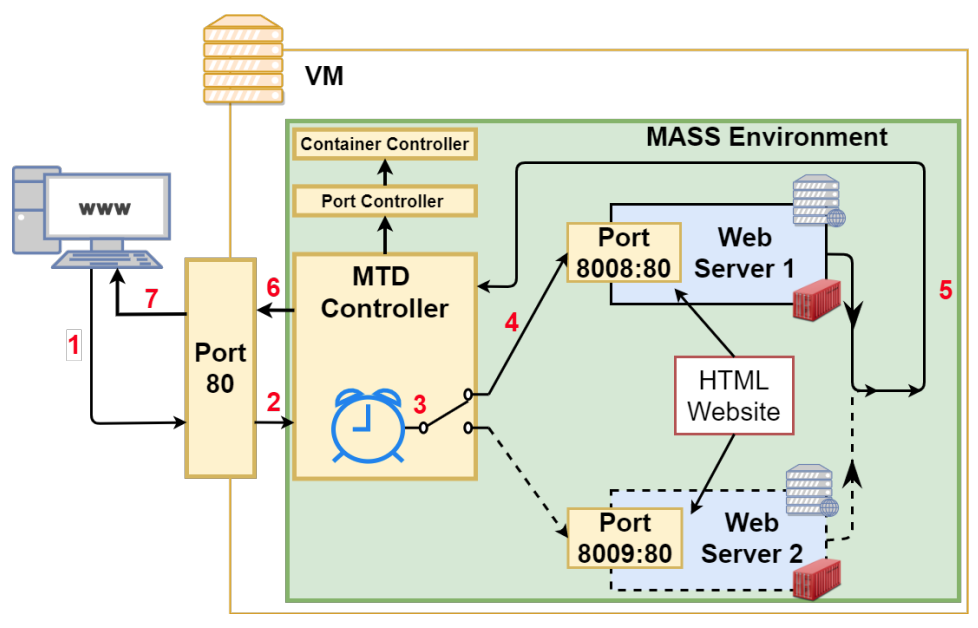
\includegraphics[width=\linewidth]{./imagenes/mass-structure.png}
    \caption{Estructura original del MASS con flujo de tráfico.\cite{MTD-DARE-DIM-MASS}}
\end{figure}

\begin{itemize}
    \item Controlador del MTD: el cual es el encargado de controlar el tiempo y activar el cambio de servidor. Soporta tanto rotación en intervalos fijos como entre un rango de tiempos.
    \item Controlador de contenedores: es el encargado de encender y matar los contenedores con los servidores.
    \item Controlador de puertos: es el encargado de controlar el \textit{firewall} para redirigir el tráfico desde el puerto 80 a el puerto interno del servidor activo (8008 y 8009). 
\end{itemize}

En la implementación realizada se han separado el controlador de contenedores del de puertos, siendo ambos controlados directamente por el controlador del MTD. Esta representación se puede ver en el siguiente diagrama de clases.

\begin{figure}[H]
    \centering
    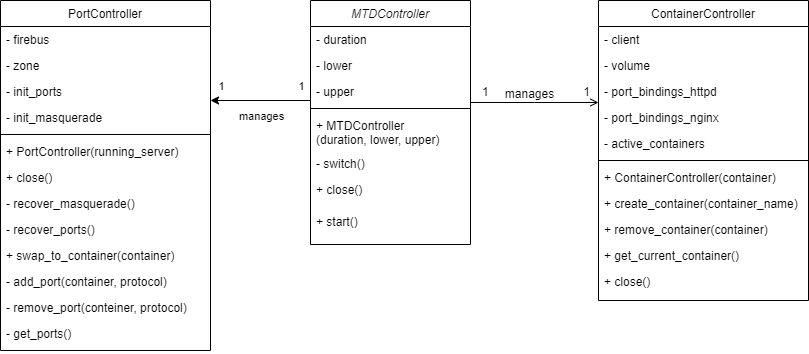
\includegraphics[width=\linewidth]{./imagenes/clases.png}
    \caption{Diagrama de clases de la implementación.}
\end{figure}


\section{Tests}
Para comprobar si la solución se ajusta a los requisitos se han desarrollado los siguientes tests:
\begin{itemize} 
    \item Uso de CPU en reposo: para ver como afecta la rotación de los servidores a el uso normal del servidor. 
    \item Rendimiento: para comprobar cuanta carga de peticiones puede soportar y como afecta al uso de CPU.
    \item Explotación: se ha explotado una vulnerabilidad en uno de los dos servidores para ver si la rotación ayuda a mitigar el tiempo de exposición.
\end{itemize}


	% % Presupuesto

	% % Conclusiones
	\chapter{Conclusiones y trabajos futuros}

En este capítulo se presentarán las conclusiones derivadas del trabajo realizado, con especial énfasis en las pruebas y los resultados obtenidos a lo largo del desarrollo del proyecto. El enfoque en las pruebas de funcionalidad, integración, rendimiento y seguridad permitió evaluar de manera exhaustiva la calidad y robustez del sistema. A partir de estas evaluaciones, se identificaron puntos fuertes y áreas de mejora en el desarrollo del proyecto.

Además de las conclusiones, se explorarán las posibles líneas de trabajo futuro que podrían ampliar o mejorar el proyecto actual. Estas propuestas incluyen mejoras en la metodología de pruebas, optimización del rendimiento bajo distintas condiciones y la implementación de nuevas características que permitan adaptarse a futuros cambios en el entorno de trabajo. Este análisis ofrece una guía para las fases posteriores, tanto en el perfeccionamiento del producto como en su ampliación a nuevas áreas de aplicación.

\section{Conclusiones}
Apache Benchmark permitió medir la capacidad del MASS bajo carga. Los resultados muestran que los servidores sometidos a la prueba (Nginx, Httpd, y las diferentes configuraciones de MASS) lograron manejar 150,000 solicitudes concurrentes sin pérdidas de peticiones. Sin embargo, al comparar los tiempos de respuesta, los servidores MASS mostraron tiempos más altos en los percentiles superiores en comparación con Nginx. Esto es esperable, ya que MASS rota entre Apache y Nginx, y dado que Apache tiene una capacidad de respuesta más baja, obtenemos tiempos de respuesta intermedios. Por lo tanto, este es un resultado esperado y positivo, ya que el sistema sigue siendo capaz de gestionar una carga elevada sin comprometer la integridad de las solicitudes o sufrir pérdidas de peticiones.

El uso de la herramienta sar para monitorizar el uso de CPU en reposo muestra diferencias notables entre las configuraciones. Mientras que Nginx y Httpd mantienen un bajo uso de CPU (~2.18\% y ~2.19\% respectivamente), las configuraciones MASS muestran un uso significativamente más alto, alcanzando hasta un promedio de 7.86\% en la configuración MASS[15,15]. Esto se debe a la naturaleza de las rotaciones periódicas de los contenedores en MASS, lo que genera mayor actividad en segundo plano incluso en estado de reposo. 

Las configuraciones de MASS mostraron una tasa de éxito de ataque significativamente más baja, oscilando entre el 44\% y el 47\%, lo que indica una mayor resistencia a este tipo de ataques, versus el 100\% que tiene el servidor HTTPD. Al estar tan cerca del 50\% se puede suponer que el ataque siempre funcionará si el servidor HTTPD es expuesto.

Por lo que en términos generales, MASS cumple con su objetivo de proporcionar un sistema capaz de gestionar altas cargas sin pérdidas de peticiones, aunque con un uso de CPU más elevado en reposo. En el caso de que uno de los servidores sea vulnerable, el sistema será vulnerable tanto tiempo como este servidor esté expuesto, lo cual es uno de los problemas intrínsecos de esta tecnología. Por tanto, el sistema demuestra ser una solución robusta y confiable, cumpliendo con los requisitos esperados en cuanto a rendimiento y seguridad y siendo autocontenido.


\section{Trabajo futuro}
Para continuar mejorando el rendimiento y la seguridad del sistema MASS, se proponen las siguientes líneas de trabajo futuro:
\begin{itemize}
    \item \textbf{Implementación de un IDS (Sistema de Detección de Intrusos) con rotación basada en eventos}: La integración de un IDS permitirá monitorear en tiempo real la actividad de los servidores y detectar posibles amenazas o comportamientos anómalos. Además, se plantea combinar este sistema de detección con una rotación híbrida basada en eventos. Esto significa que los contenedores no solo rotarán en intervalos de tiempo predefinidos, sino que también lo harán en respuesta a eventos detectados por el IDS, como intentos de ataque, picos inusuales de tráfico o cambios en los recursos del sistema. De esta manera, el sistema podrá reaccionar de forma proactiva ante posibles amenazas, fortaleciendo su capacidad de defensa sin comprometer el rendimiento. Además, se mitigaría un poco el problema de \ref{caza}, ya que se reduciría el tiempo de exposición del servidor vulnerable.
    \item \textbf{Restauración de contenedores desde snapshots}: Implementar la capacidad de restaurar contenedores desde \textit{snapshots} permitirá una recuperación rápida y eficiente en caso de fallos o ataques. Con la restauración desde snapshots, el sistema podrá volver a un estado seguro y funcional en un tiempo mínimo, mejorando la resiliencia y el rendimiento.
\end{itemize}

Estas mejoras permitirán que el sistema MASS evolucione hacia una solución más dinámica, capaz de adaptarse a situaciones de alto riesgo, garantizando la seguridad y el rendimiento de manera más efectiva.
	\chapter{Glosario}

\begin{itemize}
    \item \textbf{ACL}: Access Control List
    \item \textbf{ANCOR}: Framework for creating and managing cloud-based IT systems using a high-level abstraction (an up-to-date IT system inventory).
    \item \textbf{BDD}: Behavior Driven Development
    \item \textbf{CPU}: Central Processing Unit
    \item \textbf{CVE}: Common Vulnerabilities and Exposures
    \item \textbf{DARE}: Dynamic Application Rotation Environment for Moving Target Defense
    \item \textbf{DIM}: DARE IMproved
    \item \textbf{DoS}: Denial of Service
    \item \textbf{HTTP}: Hypertext Transfer Protocol
    \item \textbf{IPS}: Intrusion Prevention System
    \item \textbf{K8s}: Kubernetes
    \item \textbf{MASS}: Mutable Asymmetric web Server Security
    \item \textbf{MORE}: Multiple Operating System Rotational Environment MTD
    \item \textbf{MTD}: Moving Target Defense
    \item \textbf{SCIT}: Self Cleansing Intrusion Tolerance
    \item \textbf{SLA}: Service Level Agreement
    \item \textbf{SO}: Sistema Operativo
    \item \textbf{VM}: Virtual Machine
    \item \textbf{WAF}: Web Application Firewall
    \item \textbf{SDN}: Software Defined Network
    \item \textbf{OCI}: Open Container Initiative
    \item \textbf{PEP}: Python Enhancement Proposals
    \item \textbf{RCE}: Remote Code Execution
    \item \textbf{SAR}: System Activity Report
  \end{itemize}
  

	% Trabajos futuros


	
	\newpage
	\bibliography{bibliografia}
	\bibliographystyle{plain}
	
\end{document}

